\clearpage
\section{Appendix}
\subsection{Training-Inference Mismatch Analysis in RL}
\label{rl_appendix}
% 需在导言区加入: \usepackage{subcaption}
% 若图片在 figs/ 下，将 figures/ 改为 figs/
% \begin{figure}[h]
%     \centering
%     % 第一排：三图
%     \begin{subfigure}[b]{0.32\linewidth}
%         \centering
%         \includegraphics[width=\linewidth]{figs/actor_entropy.png}
%         \label{fig:metrics:a}
%     \end{subfigure}
%     \hfill
%     \begin{subfigure}[b]{0.32\linewidth}
%         \centering
%         \includegraphics[width=\linewidth]{figs/actor_grad_norm.png}
%         \label{fig:metrics:b}
%     \end{subfigure}
%     \hfill
%     \begin{subfigure}[b]{0.32\linewidth}
%         \centering
%         \includegraphics[width=\linewidth]{figs/critic_score_mean.png}
%         \label{fig:metrics:c}
%     \end{subfigure}

%     \vspace{0.8em}

%     % 第二排：居中两个图片
%     \makebox[\textwidth][c]{
%         \begin{subfigure}[b]{0.32\linewidth}
%             \centering
%             \includegraphics[width=\linewidth]{figs/training_filtered_entropy_samples.png}
%             \label{fig:metrics:d}
%         \end{subfigure}
%         \hspace{0.06\linewidth}
%         \begin{subfigure}[b]{0.32\linewidth}
%             \centering
%             \includegraphics[width=\linewidth]{figs/training_rollout_probs_diff_mean.png}
%             \label{fig:metrics:e}
%         \end{subfigure}
%     }

%     \caption{Training metrics comparison in RL.}
%     \label{fig:metrics}
% \end{figure}

\begin{figure}[h]
    \centering
    % 一排四图（均匀分布）
    \begin{subfigure}[b]{0.24\linewidth}
        \centering
        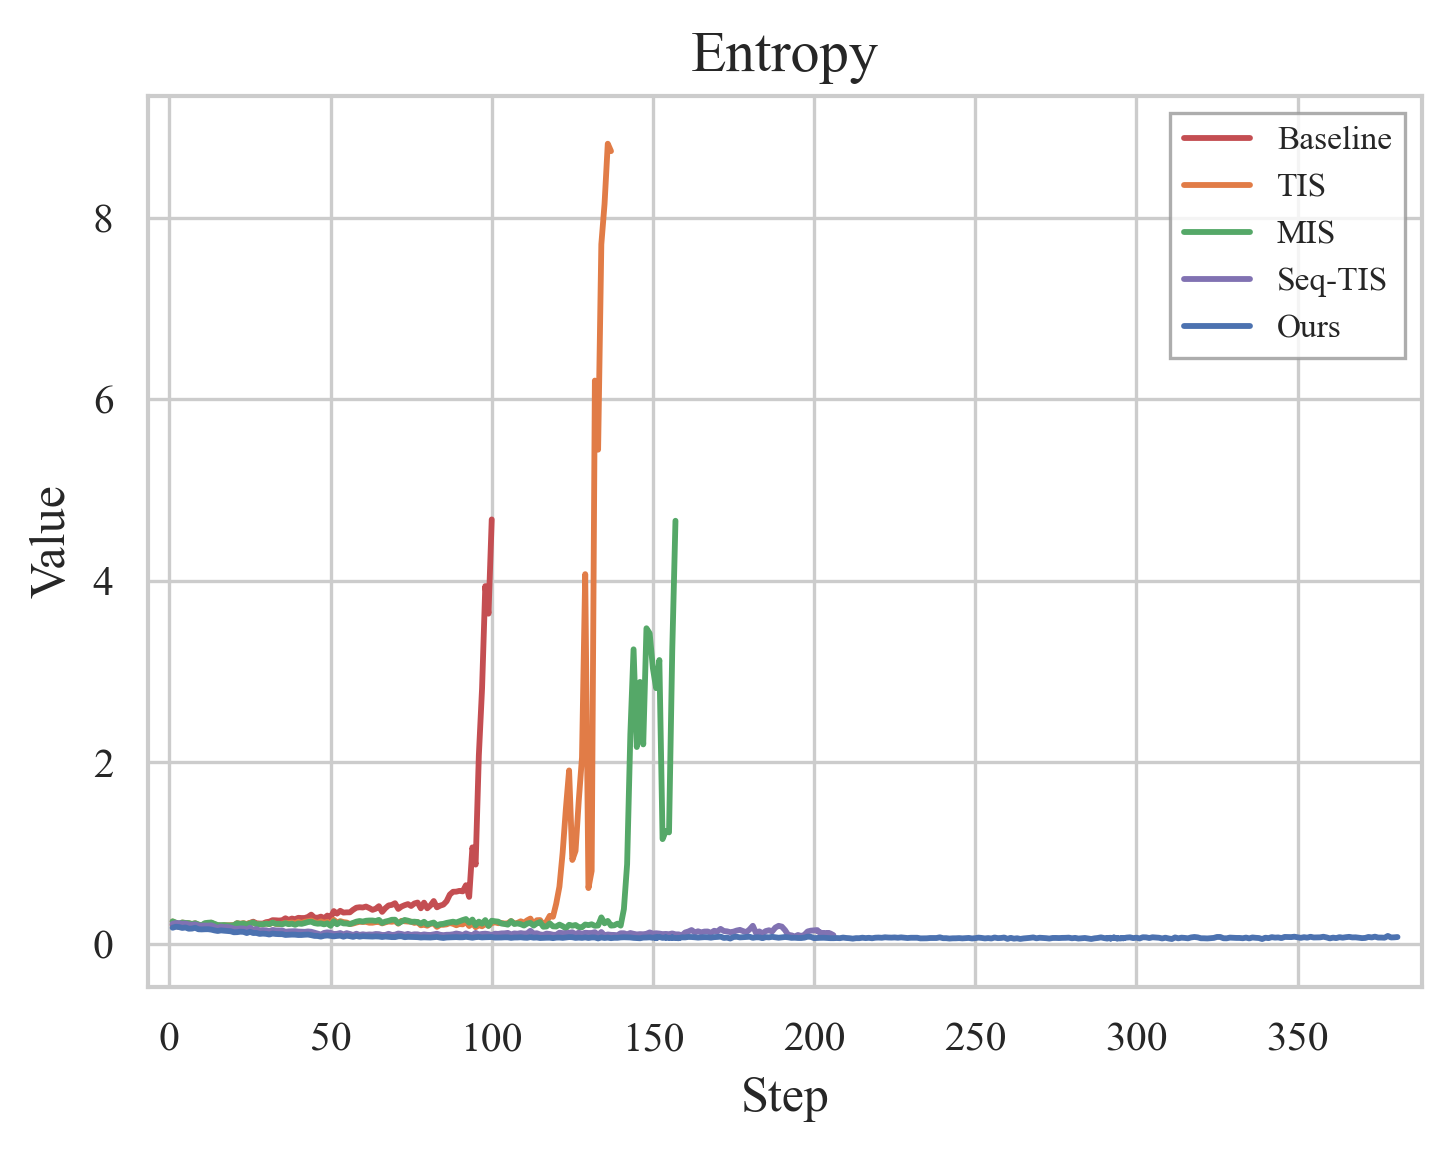
\includegraphics[width=\linewidth]{figs/actor_entropy_v2.png}
        \label{fig:metrics:a}
    \end{subfigure}
    \hfill  % 自动填充空白空间
    \begin{subfigure}[b]{0.24\linewidth}
        \centering
        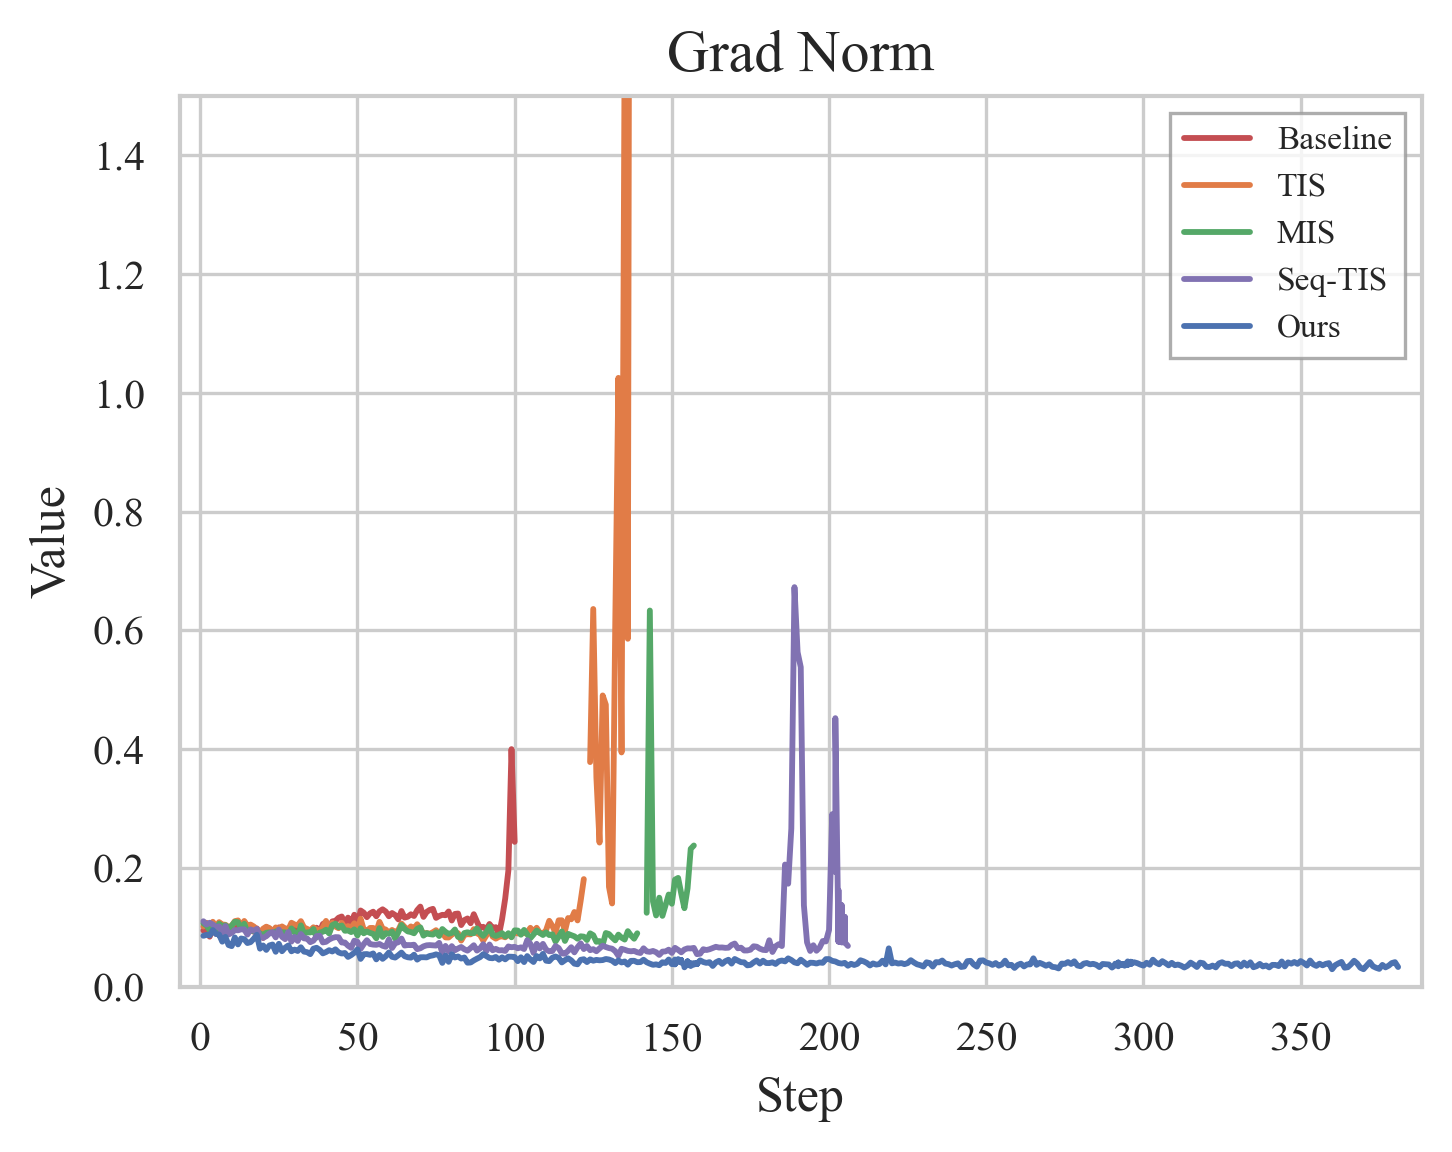
\includegraphics[width=\linewidth]{figs/actor_grad_norm_v2.png}
        \label{fig:metrics:b}
    \end{subfigure}
    \hfill
    \begin{subfigure}[b]{0.24\linewidth}
        \centering
        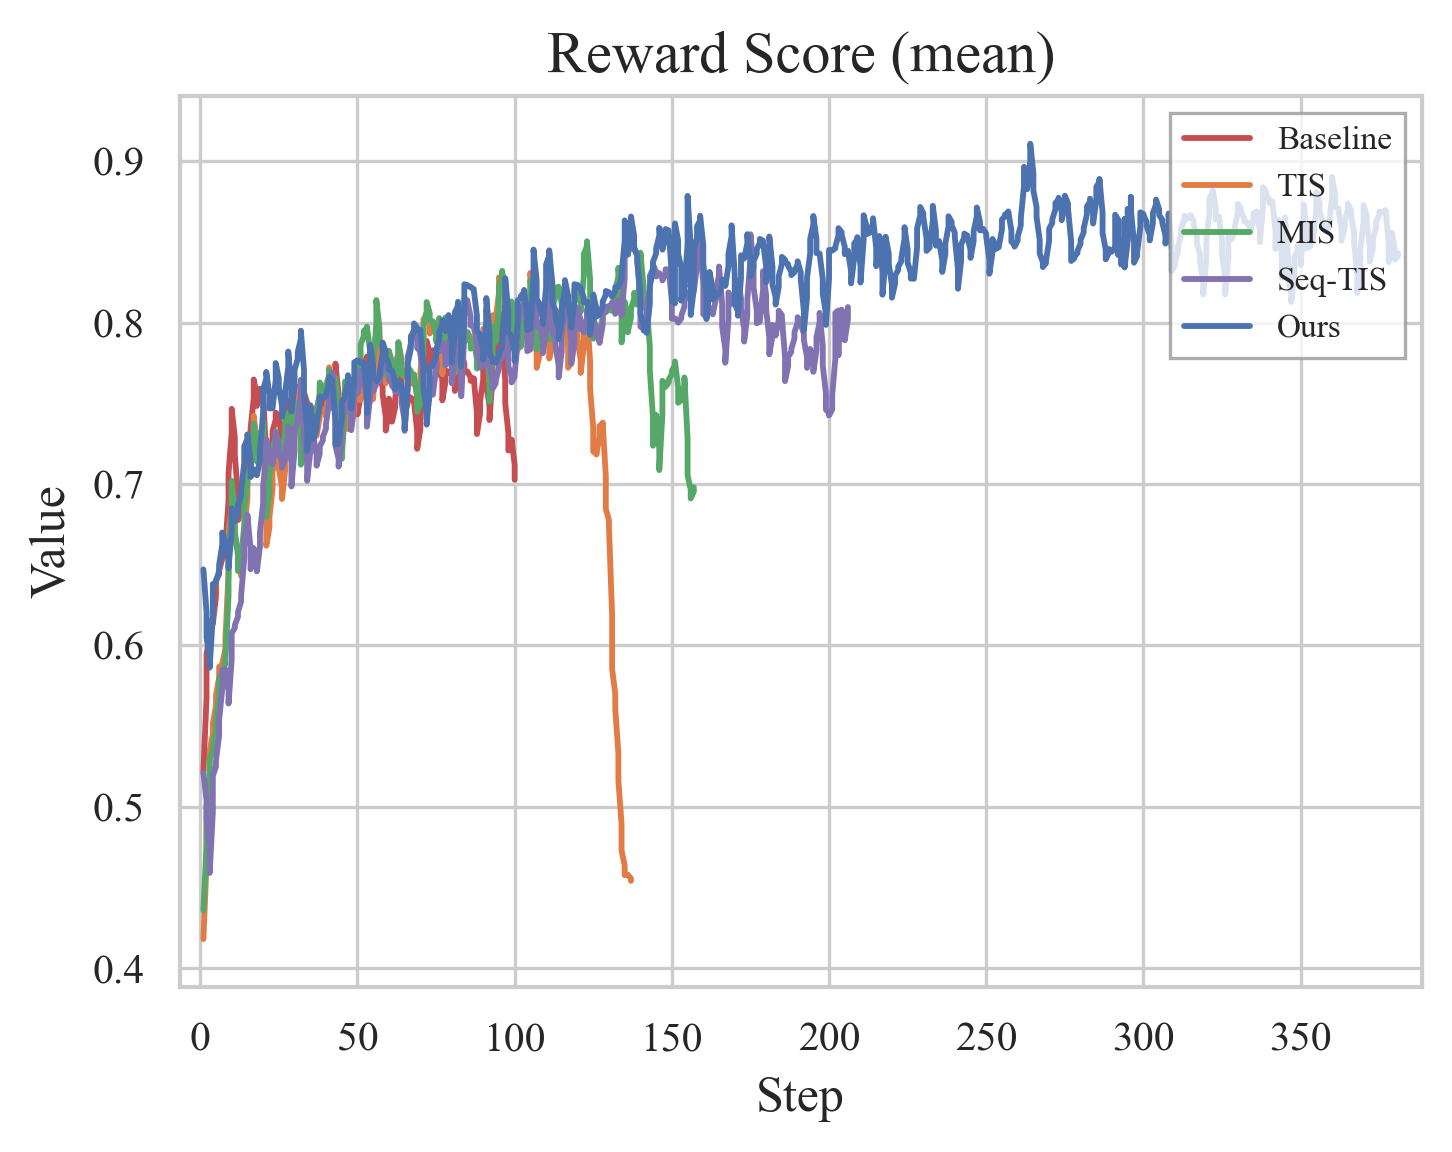
\includegraphics[width=\linewidth]{figs/critic_score_mean_v2.png}
        \label{fig:metrics:c}
    \end{subfigure}
    \hfill
    \begin{subfigure}[b]{0.24\linewidth}
        \centering
        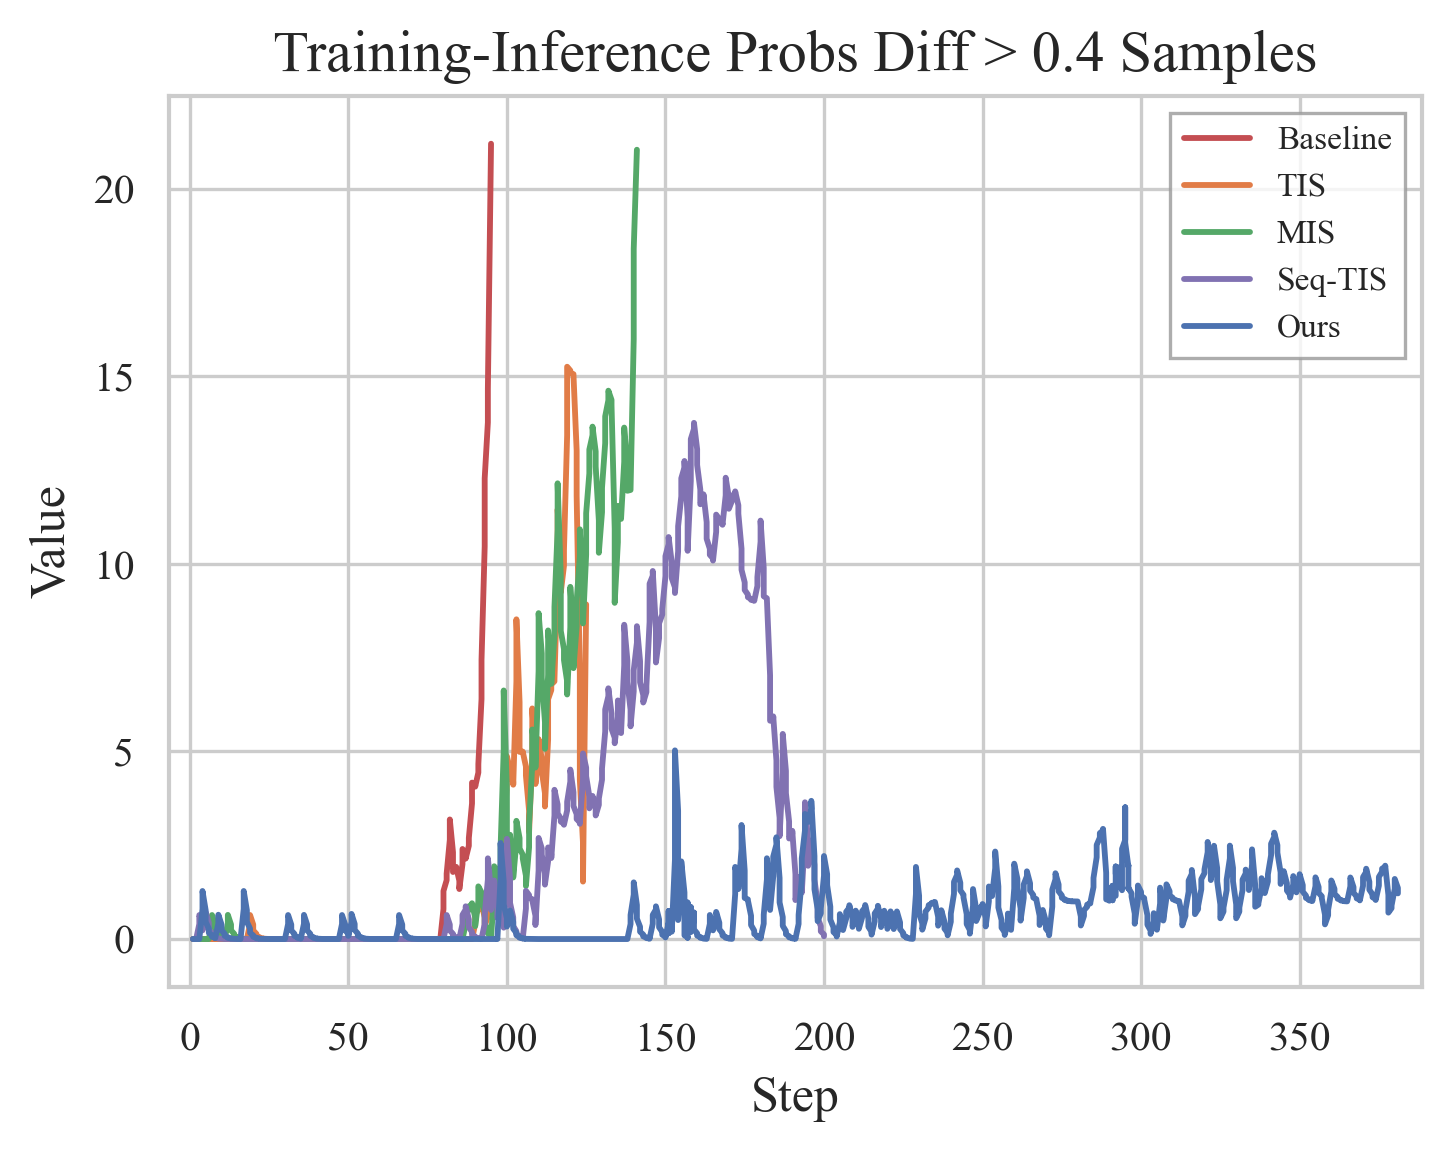
\includegraphics[width=\linewidth]{figs/training_filtered_entropy_samples_v2.png}
        \label{fig:metrics:d}
    \end{subfigure}

    \caption{Training metrics comparison in RL.}
    \label{fig:metrics_rl}
\end{figure}

During RL training, we identified a critical phenomenon: sequence collapse is frequently triggered by severe training-inference mismatch in only a few or even a single token within a sequence. A token may have a probability exceeding 
$0.4$ under the sampling policy $\pi_{\text{sampler}}$, while its estimated probability under the training policy $\pi_{\text{actor}}$ can be as low as $10^{-2}$, whereas the average probability difference for the remaining tokens in the same sequence is on the order of $10^{-3}$. Such anomalous tokens have a catastrophic effect on overall sequence quality. They represent extremely low-probability noise that would normally be difficult to rollout but infiltrate the data due to hardware or numerical precision mismatches. More critically, subsequent generations contingent on these noisy tokens become unreliable, leading to error propagation throughout the sequence. Fig.~\ref{fig:metrics_rl} shows the number of samples in a batch where the training-inference probability divergence exceeds $0.4$ for at least one token. As illustrated, entropy explosion, gradient norm surges, and increasing training-inference policy divergence exhibit a positive correlation. This chain of factors ultimately leads to a decline in reward. 

To mitigate this issue, we experimented with several importance sampling correction techniques, including Truncated Importance Sampling (TIS)\cite{yao2025offpolicy} and Multiple Importance Sampling (MIS)\cite{liu2025speed}. As shown in Fig.~\ref{fig:metrics_rl}, these approaches merely delayed the onset of entropy explosion by a few training steps without addressing the fundamental problem. 

Some sequence-level correction methods\cite{liu-li-2025-rl-collapse} may also fail in this scenario and lead to a decrease in reward. The extreme divergence of a few anomalous tokens can be averaged out by the ratios of the many normal tokens in the sequence. 
Therefore, we adopt a more fundamental and direct intervention strategy, the threshold $\delta$ directly to the per-token absolute probability difference $|\pi_{\text{sampler}} - \pi_{\text{actor}}|$. This enables our filter to directly detect and pinpoint the finest-grained, token-level inconsistencies. By applying these strict filtering strategies, we effectively prevented noisy data from entering the training process.

\subsection{Experimental Analysis for RL}
\label{rl_exp}
In this experiment, we use Qwen-7B as the language backbone to validate the effectiveness of discretized RL. Except for LLM backbone, all other model architectures and configurations remain consistent with those used in the pretrained model. 
We evaluate the performance on both image understanding and image generation tasks. 

For the image understanding task, we conduct RL training using the open-source datasets VIRL39K~\cite{DBLP:journals/corr/abs-2504-08837} and Orsta-Data-47k~\cite{ma2025one}, along with in-house data. 
We merge and deduplicate the datasets based on image hash and prompt, perform four rollouts using the base model, and remove instances that are either entirely correct or entirely incorrect. Ultimately, we retain approximately 30K RL data samples. 
For the image generation task, we collect approximately 40K data samples, with each prompt potentially associated with multiple reward scores. 
Detailed performance results are presented in Table~\ref{rl_und}.

\begin{table}[htbp]
\vspace{-4pt}
\begin{center}
\small
\setlength{\tabcolsep}{8pt} % 列间距
\renewcommand{\arraystretch}{0.9}
\caption{Image Understanding and image generation performance based on Qwen-7B.}
\resizebox{0.95\textwidth}{!}{
\begin{tabular}{lccccccc}
    \toprule
    \multicolumn{1}{c}{} 
    & \multicolumn{4}{c}{\textbf{STEM}} 
    & \multicolumn{3}{c}{\textbf{General}} \\
    \cmidrule(lr){2-5} \cmidrule(lr){6-8}
    Dataset & MMMU & MMMU-Pro & MathVista & MathVision & MMStar  & RealWorldQA & MMVP \\
    \midrule
    baseline & 64.22 & 51.27 & 80.30 & 49.28 & 66.33 & 66.01  & 73.33 \\
    RL       & \textbf{66.45} & \textbf{53.58} & 81.90 & \textbf{53.52} & \textbf{71.13} &\textbf{72.54}  & 74.66 \\
    \midrule[\heavyrulewidth]
    \multicolumn{8}{c}{\textbf{OCR \& Doc}} \\
    \midrule
    Dataset & CharXiv$_\text{DQ}$  & CharXiv$_\text{RQ}$ & InfoVQA  & ChartQA & AI2D & \multicolumn{2}{c}{OmniDocBench(zh / en)$\downarrow$}    \\
    baseline & 85.45  & 51.8 & 81.69 & 88.56 & 81.57 & 0.187 & 0.256   \\
    RL   & \textbf{87.35}  & \textbf{56.7} & \textbf{83.85} & \textbf{92.08} & \textbf{85.13} & \textbf{0.169} & 0.266 \\
    \midrule[\heavyrulewidth]
    \multicolumn{8}{c}{\textbf{GenEval}} \\
    \midrule
    Dataset & Overall & single\_obj & two\_obj & counting & colors & position & color\_attr   \\
    baseline & 83.94 & 100.00 & 92.71  &  71.25 & 92.74  &  74.75 & 72.19    \\
    RL  &  \textbf{87.33} &  99.69 & 93.18 & \textbf{78.75}  &   94.15 & \textbf{81.50} &  \textbf{76.75}   \\
    \bottomrule
    \label{rl_und}
\end{tabular}
}
\vspace{-8pt}
\end{center}
\end{table}

% \begin{tabular}{lcccccccc}
%     \toprule
%     \multicolumn{1}{c}{} 
%     & \multicolumn{4}{c}{\textbf{Stem}} 
%     & \multicolumn{4}{c}{\textbf{General}} \\
%     \cmidrule(lr){2-5} \cmidrule(lr){6-9}
%     Dataset & MMMU & MMMU-Pro & MathVista & MathVision & RealWorldQA & MMStar & MMVP & SEEDBench \\
%     \midrule
%     baseline & 64.22 & 51.27 & 80.30 & 49.28 & 66.01 & 66.33 & 73.33 & 76.06 \\
%     RL       & \textbf{66.45} & \textbf{53.58} & 81.90 & \textbf{53.52} & \textbf{72.54} & \textbf{71.13} & 72.66 & 76.11 \\
%     \midrule[\heavyrulewidth]
%     \multicolumn{9}{c}{\textbf{OCR \& Doc}} \\
%     \midrule
%     Dataset & OmniDocBench$_\text{en}$$\downarrow$ & OmniDocBench$_\text{zh}$$\downarrow$ & CharXiv$_\text{DQ}$  & CharXiv$_\text{RQ}$ & InfoVQA  & ChartQA & AI2D & OCRBenchV2$_\text{en}$  \\
%     baseline & 0.187 & 0.256 & 85.45  & 51.8 & 81.69 & 88.56 & 81.57  & 0.565  \\
%     RL       & \textbf{0.169} & 0.266  & \textbf{87.35}  & \textbf{56.7} & \textbf{83.85} & \textbf{92.08} & \textbf{85.13} & 0.565 \\
%     \midrule[\heavyrulewidth]
%     \multicolumn{9}{c}{\textbf{Geneval}} \\
%     \midrule
%     Dataset & Overall & single\_obj & two\_obj & counting & colors & position & color\_attr   \\
%     baseline & 83.94 & 100.00 & 92.71  &  71.25 & 92.74  &  74.75 & 72.19    \\
%     RL  &  \textbf{87.33} &  99.69 & 93.18 & \textbf{78.75}  &   94.15 & \textbf{81.50} &  \textbf{76.75}   \\
%     \bottomrule

    
%     \label{rl_und}
% \end{tabular}
% \end{center}
% \end{table}

RL exhibits significant improvements across the STEM, General VQA, and OCR benchmarks. For example, scores on datasets such as MMMU and MathVision show notable gains compared with the baseline model, demonstrating a substantial enhancement in the model's multi-step reasoning and problem-solving capabilities. Furthermore, for general VQA and OCR tasks such as RealWorldQA, MathStar, and ChartQA, the model also achieves significant improvements of around 5\%, indicating a comprehensive boost in its generalization capability. On the GenEval evaluation set for image generation, our model also achieves notable performance gains: counting accuracy improves by 7.50\%, position accuracy by 6.75\%, and color attribute accuracy by 4.56\%. These results highlight the effectiveness of reinforcement learning driven by reward feedback.

\subsection{Discrete Quantization Strategy}

% 使用 \noindent 防止 minipage 缩进导致排版错乱
\noindent
% 第一个 minipage，放置图片
\begin{minipage}[c]{0.35\linewidth} % [c] 表示垂直居中对齐，宽度占行宽的 45%
    \centering
    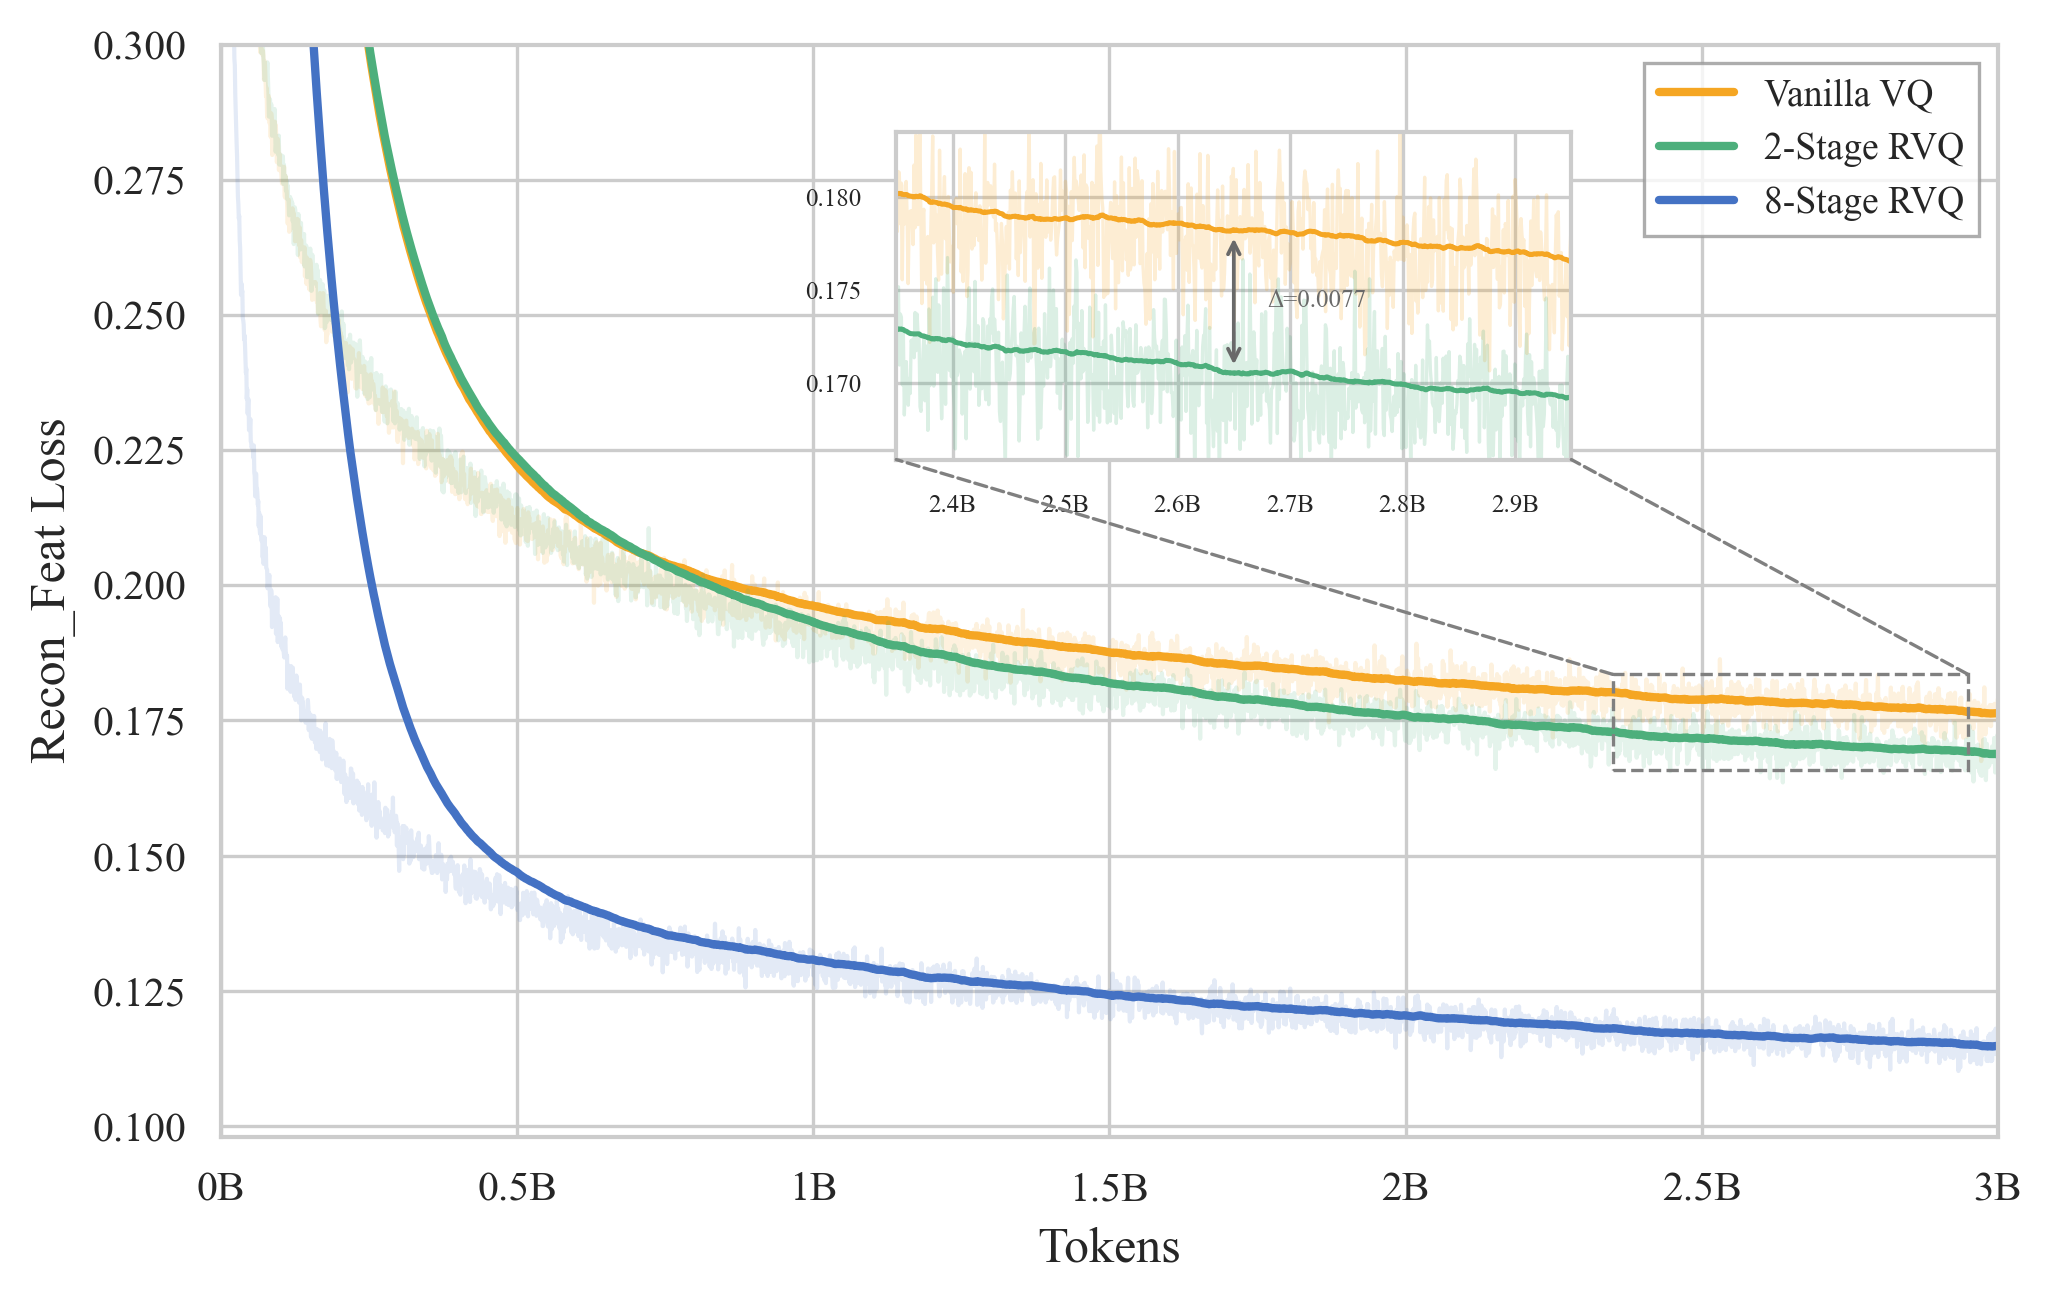
\includegraphics[width=\linewidth]{figs/rvq_loss.png} 
    \captionof{figure}{Comparison of feature reconstruction loss across different discrete quantization strategies.}
    \label{fig:rvq_loss}
\end{minipage}
% 这里使用 \hfill，会自动填满中间的空白，将文字推向右侧
\hfill
% 第二个 minipage，放置文字
\begin{minipage}[c]{0.60\linewidth} % 文字宽度占行宽的 50%，与图片宽度之和加上间隙略小于 1
\small % 如果文字较多，可以考虑用小号字体让图片看起来相对更大一些（可选）
To select a discrete quantization strategy that minimizes information loss, we utilize feature reconstruction loss as a proxy task to evaluate the method's information retention capabilities. As shown in Fig.~\ref{fig:rvq_loss}, the two-stage RVQ outperforms the vanilla VQ slightly. Furthermore, when scaling the RVQ to eight stages, the feature reconstruction loss decreases significantly. This demonstrates that the residual mechanism and compositionality of RVQ are essential for achieving discrete quantization with minimal information loss. Empirical validation confirms that the eight-stage RVQ achieves sufficiently low information loss without imposing excessive computational overhead, fully meeting our requirements. Consequently, we adopt it as the default setting for our model.
\vspace{-3pt}
\end{minipage}

% 并排结构结束，接下来的内容会自动换行到下方
\vspace{1em} % 添加一点垂直间距让排版更好看


\subsection{Vision Understanding and Generation under DiNA}


In the autoregressive modeling process under DiNA, as in Fig.~\ref{fig:rvq_loss}, we effectively balance performance and efficiency through multi-level encoding and decoding. During the understanding phase, visual signals are encoded into hierarchical discrete tokens, which are then additive over the levels before being fed into the large language model (LLM), ensuring that information from all levels is fully utilized. During the generation phase, hidden representations are passed to the DepthTransformer, which decodes them into multi-level tokens. This entire process is completed in a single autoregressive step, enabling efficient parallel decoding while maintaining high-quality generation. This approach allows visual understanding and generation to proceed seamlessly within a unified framework, overcoming the information loss and computational bottlenecks seen in traditional models.


\begin{figure}[hbtp]
    \centering
    \includegraphics[width=0.8\linewidth]{figs/UMM.pdf}
    \caption{A unified tokenizer and detokenizer for both understanding and generation within the DiNA paradigm.}
    \label{fig:dnavit_umm}
\end{figure}






% \begin{figure}
%     \centering
%     \includegraphics[width=0.8\linewidth]{figs/ocr_ood_test_case2.pdf【todo：lxy 要改】}
%     \caption{Micro-text Recognition. Extraction result with reasoning progress of tiny text on the box that is almost unreadable for humen eyes.}
%     \label{fig:placeholder}
% \end{figure}


% \begin{figure}
%     \centering
%     \includegraphics[width=1.0\linewidth]{figs/3-ocr-newspaper.jpg}
%     \caption{This constitutes a highly challenging case due to the intricate layout of the newspaper document. Our model successfully extracts the query-relevant local information in its entirety, despite exhibiting occasional word-level inaccuracies in the multi-column text extraction.}
%     \label{fig:placeholder}
% \end{figure}



% \begin{figure}[htbp]
%     \centering
%     % --- 上部分：原图 ---
%     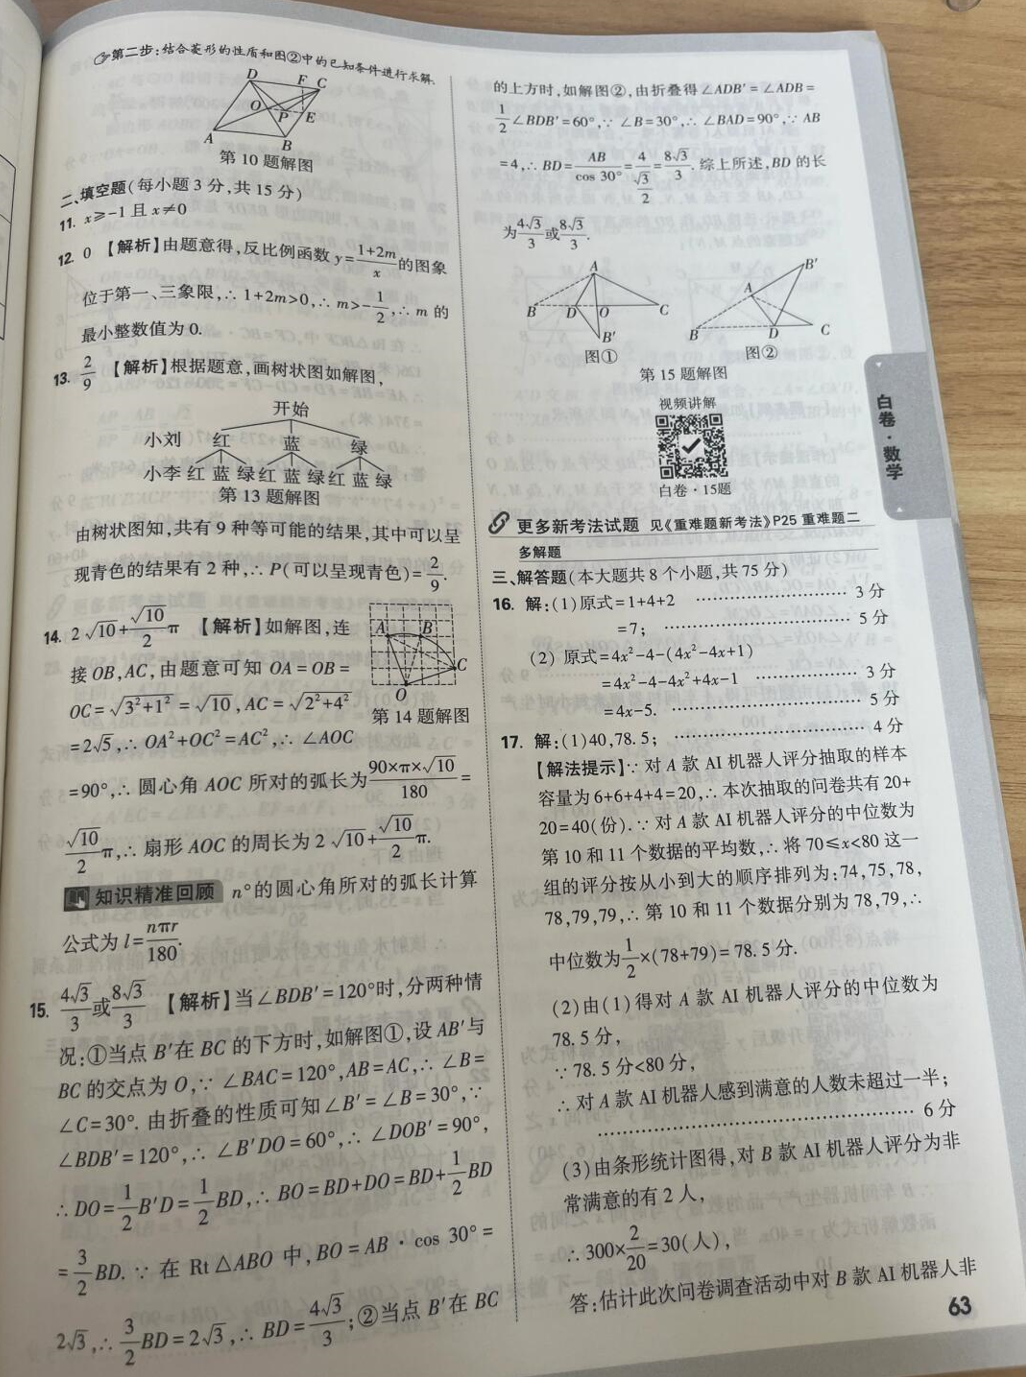
\includegraphics[width=0.27\textwidth]{figs/ocr_case_latex.png} 
%     \vspace{0.5cm} % 图文间距
    
%     % --- 下部分：模型输出的 Markdown/LaTeX 结果 ---
%     \begin{tcolorbox}[
%         enhanced, 
%         breakable, 
%         colback=gray!5, 
%         colframe=gray!50!black, 
%         title=\textbf{Model Output: Text and LaTeX Formulas}, 
%         fonttitle=\bfseries,
%         attach boxed title to top left={yshift=-2mm, xshift=5mm},
%         boxed title style={colback=gray!70!black}
%     ]
%     % ==========================================
%     \scriptsize % 设置小字号
%     \linespread{1.3}\selectfont % 【核心修复】原生设置行距，无需宏包
%     % ==========================================
    
%     \begin{CJK*}{UTF8}{gbsn}
%     A：A=$\pi r^2$第二步：结合菱形的性质和图2中的已知条件进行求解
    
%     第10题解图
    
%     \textbf{二、填空题(每小题3分，共15分)}
    
%     11. $ x \ge -1 $ 且 $ x \neq 0 $
    
%     12. 【解析】由题意得，反比例函数 $ y = \frac{1+2m}{x} $ 的图象位于第一、三象限， $ \therefore 1+2m > 0, \therefore m > -\frac{1}{2}, \therefore m $ 的最小整数值为 0.
    
%     13. $ \frac{2}{9} $ \\
%     【解析】根据题意，画树状图如解图， \\
%     小李红蓝绿红蓝绿红蓝绿 \\
%     第13题解图 \\
%     由树状图知，共有9种等可能的结果，其中可以呈现青色（绿色）的结果有2种， $ \because P $ （可以呈现青色）= $ \frac{2}{9} $ .
    
%     14. $ 2\sqrt{10}+\frac{\sqrt{10}}{2}\pi $ \\
%     【解析】如解图，连接OB，AC，由题意可知 $ OA=OB=OC=\sqrt{3^{2}+1^{2}}=\sqrt{10} $ ， $ AC=\sqrt{2^{2}+4^{2}}=2\sqrt{5} $ ， $ OA^{2}+OC^{2}=AC^{2} $ ， $ \therefore \angle AOC=90^{\circ} $ ， $ \therefore $ 圆心角AOC所对的弧长为 $ \frac{90\times\pi\times\sqrt{10}}{180}=\frac{\sqrt{10}}{2}\pi $ ，扇形AOC的周长为 $ 2\sqrt{10}+\frac{\sqrt{10}}{2}\pi $ . \\
%     知识精准回顾 $ n^{\circ} $ 的圆心角所对的弧长计算公式为 $ l = \frac{n\pi r}{180} $ .
    
%     15. $ \frac{4\sqrt{3}}{3} $ 或 $ \frac{8\sqrt{3}}{3} $ \\
%     【解析】当 $ \angle B D B^{\prime}=120^{\circ} $ 时，分两种情况：①当点 $ B^{\prime} $ 在BC的下方时，如解图①，设AB与 $ B C^{\prime} $ 的交点为O， $ \because \angle BAC=120^{\circ} $ ，$ AB=AC $， $ \therefore \angle B=\angle C=30^{\circ} $ . 由折叠的性质可知 $ \angle B^{\prime}=\angle B=30^{\circ} $ ， $ \angle D B B^{\prime}=120^{\circ} $ ， $ \angle B^{\prime} D O=60^{\circ} $ ， $ \angle D O B^{\prime}=90^{\circ} $ ， $ \therefore D O=\frac{1}{2}B^{\prime}D=\frac{1}{2}B D $ ， $ \therefore B O=B D+D O=B D+\frac{1}{2}B D=\frac{3}{2}B D $ . $ \therefore $ 在Rt$\triangle$ABO中，$ BO=AB\cdot\cos 30^{\circ}=\frac{3}{2}BD $ ；②当点 $ B^{\prime} $ 在BC上方时，如解图②，由折叠得 $ \angle ADB^{\prime}=\angle ADB=\frac{1}{2}\angle BDB^{\prime}=60^{\circ} $ ， $ \therefore \angle B=30^{\circ} $ ， $ \therefore \angle BAD=90^{\circ} $ ， $ \therefore AB=4 $ ， $ \therefore BD=AB\cos 30^{\circ}=\frac{4}{3}\times\frac{8\sqrt{3}}{3}=\frac{4\sqrt{3}}{3} $ 或 $ \frac{8\sqrt{3}}{3} $ .
    
%     第15题解图 \\
%     视频讲解 \\
%     白卷·数学 \\
%     更多新考法试题见《重难题新考法P25重难题二》
    
%     \textbf{三、解答题(本大题共8小题，共75分)}
    
%     16.解:(1)原式=$1+4+2=7$; \\
%     (2)原式=$ 4x^{2}-4-(4x^{2}-4x+1)=4x^{2}-4-4x^{2}+4x-1=4x-5 $.
    
%     17. 解: (1)40,78.5; \\
%     【解题提示】:对A款AI机器人评分抽取的样本容量为$6+6+4+4+20$,本次抽取的问卷共有$20+6+6+4+4+20=40$(份).对A款AI机器人评分的中位数为20,将$70 \le x < 80$这一组的评分按从小到大的顺序排列为:$74,75,78,78,79,79$,第10和11个数据分别为$78,79$.中位数为$\frac{1}{2}\times(78+79)=78.5$分. \\
%     (2)由(1)得对A款AI机器人评分的中位数为78.5分, \\
%     $ \because 78.5 $分$ < 80 $分, \\
%     对A款AI机器人感到满意的人数未超过一半; \\
%     (3)由条形统计图得,对B款AI机器人评为非常满意的有2人, \\
%     $ \therefore 300\times\frac{2}{20}=30 $ (人), \\
%     答:估计此次问卷调查活动中对B款AI机器人非

%     63
%     \end{CJK*}
%     \end{tcolorbox}
    
%     \caption{Qualitative results of mathematical text and formula recognition.}
%     \label{fig:math_ocr_case}
% \end{figure}

% ====== 注意：这里不再有 \begin{figure} ======

% ====== 注意：这里不再有 \begin{figure} ======

\vspace{1em} % 和上面的正文留出一点空隙

\noindent\begin{minipage}{\textwidth}
\subsection{Qualitative Examples}
\vspace{1em}
% \begin{figure}[p] % [p] 强制它尝试单独占一页，也可以用 [htbp]
\centering

\begin{tcolorbox}[
    enhanced, 
    % 绝对不能加 breakable！
    colback=gray!2, 
    colframe=gray!50!black, 
    title=\textbf{Dense Mathematical OCR}, 
    fonttitle=\bfseries,
    attach boxed title to top left={yshift=-2mm, xshift=5mm},
    boxed title style={colback=gray!70!black},
    boxsep=2mm
]

\scriptsize 
\linespread{1.4}\selectfont 

\begin{CJK*}{UTF8}{gbsn}

% --- 左侧大盒子：包含【图片】和【前半部分文字】 ---
\begin{minipage}[t]{0.48\textwidth}
    \vspace{0pt} 
    
    \centering
    % 限制图片高度，防止撑破页面
    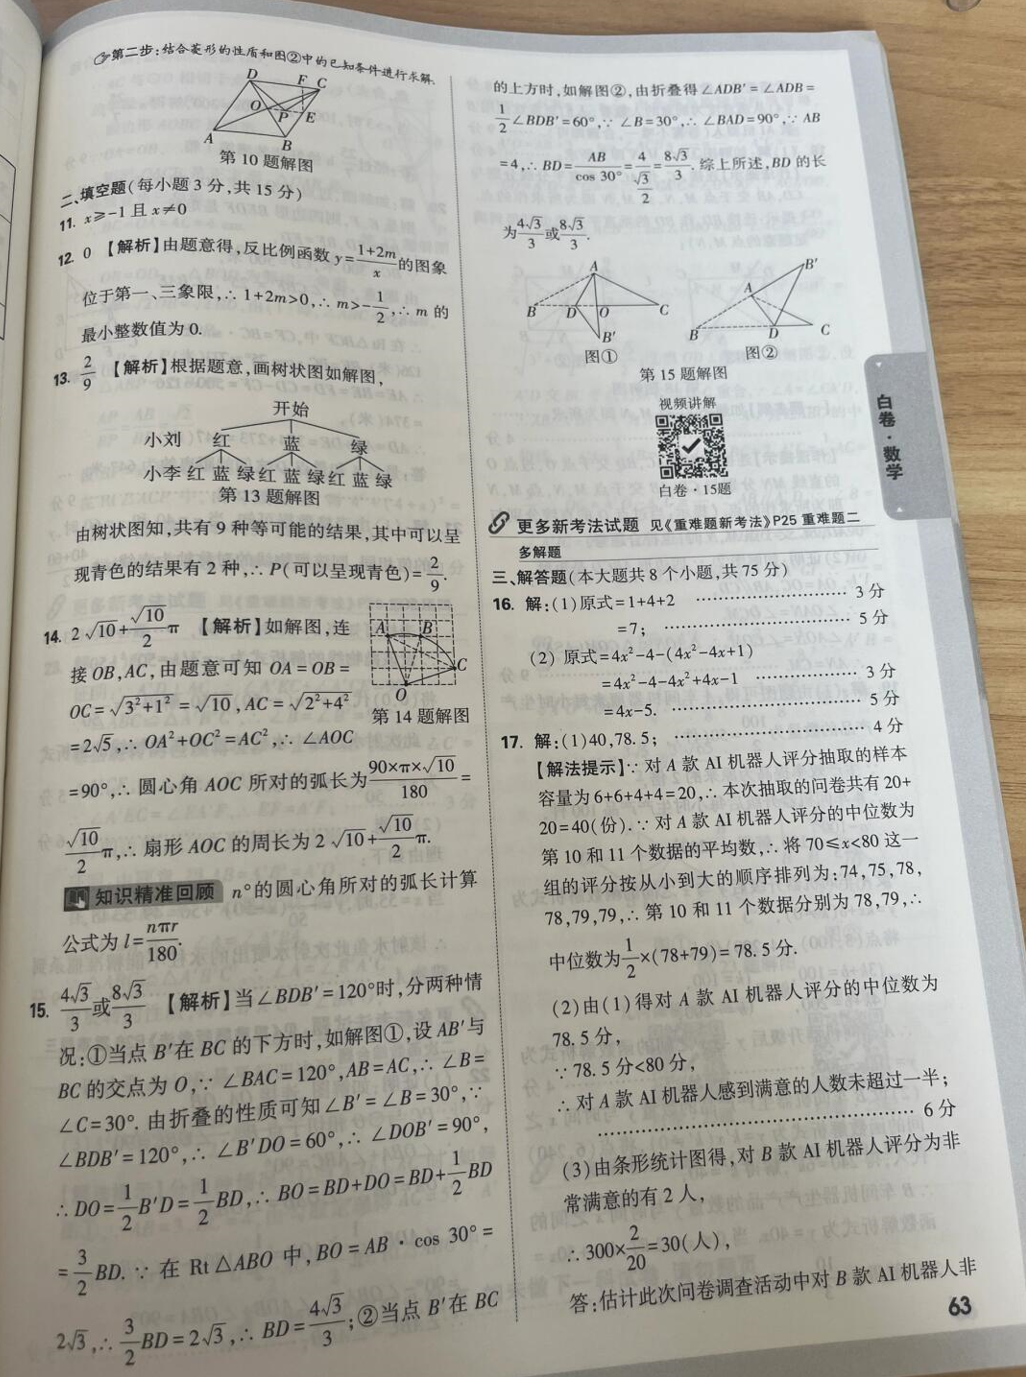
\includegraphics[width=\textwidth, height=0.45\textheight, keepaspectratio]{figs/ocr_case_latex.png}
    
    \vspace{2ex} 
    
    \raggedright 
    
    % 这里的悬挂缩进逻辑：第一行不缩进（Q：在开头），从第二行开始缩进 1.5em
    \hangindent=1.5em
    \hangafter=1
    \textbf{Q: }提取文档图片中正文的所有信息用markdown格式表示，表格用html格式表达，文档中公式用latex格式表示，按照阅读顺序组织进行解析。
    
    \vspace{1.5ex} % 保持和 A 部分的间距
    
    \vspace{1.5ex}
    
    \textbf{A: } \textit{[Model Output]} \\[0.5ex]
    \setlength{\leftskip}{1.5em} 
    
    第二步：结合菱形的性质和图2中的已知条件进行求解 \\[1ex]
    第10题解图 \\[1ex]
    \verb|##| 二、填空题(每小题3分，共15分) \\[0.5ex]
    11. $ x \ge -1 $ 且 $ x \neq 0 $ \\[0.5ex]
    12. 【解析】由题意得，反比例函数 $ y = \frac{1+2m}{x} $ 的图象位于第一、三象限， $ \therefore 1+2m > 0 $, $ \therefore m > -\frac{1}{2} $, $ \therefore m $ 的最小整数值为 0. \\[0.5ex]
    13. $ \frac{2}{9} $ \\
    【解析】根据题意，画树状图如解图， \\
    小李红蓝绿红蓝绿红蓝绿 \\
    第13题解图 \\
    由树状图知，共有9种等可能的结果，其中可以呈现青色（绿色）的结果有2种， $ \because P $ （可以呈现青色）= $ \frac{2}{9} $ .
    
    \vspace{1em} 
\end{minipage}%
\hfill 
% --- 右侧大盒子：包含【后半部分文字】 ---
\begin{minipage}[t]{0.48\textwidth}
    \vspace{0pt} 
    \raggedright 
    \setlength{\leftskip}{1.5em} 
    
    14. $ 2\sqrt{10}+\frac{\sqrt{10}}{2}\pi $ \\
    【解析】如解图，连接OB，AC，由题意可知 $ OA=OB=OC=\sqrt{3^{2}+1^{2}}=\sqrt{10} $ ， $ AC=\sqrt{2^{2}+4^{2}}=2\sqrt{5} $ ， $ OA^{2}+OC^{2}=AC^{2} $ ， $ \therefore \angle AOC=90^{\circ} $ ， $ \therefore $ 圆心角AOC所对的弧长为 $ \frac{90\times\pi\times\sqrt{10}}{180}=\frac{\sqrt{10}}{2}\pi $ ，扇形AOC的周长为 $ 2\sqrt{10}+\frac{\sqrt{10}}{2}\pi $ . \\
    知识精准回顾 $ n^{\circ} $ 的圆心角所对的弧长计算公式为 $ l = \frac{n\pi r}{180} $ . \\[1.5ex]
    
    15. $ \frac{4\sqrt{3}}{3} $ 或 $ \frac{8\sqrt{3}}{3} $ \\
    【解析】当 $ \angle B D B^{\prime}=120^{\circ} $ 时，分两种情况： \\
    ①当点 $ B^{\prime} $ 在BC的下方时，如解图①，设AB与 $ B C^{\prime} $ 的交点为O， $ \because \angle BAC=120^{\circ} $ ，$ AB=AC $， $ \therefore \angle B=\angle C=30^{\circ} $ . 由折叠的性质可知 $ \angle B^{\prime}=\angle B=30^{\circ} $ ， $ \angle D B B^{\prime}=120^{\circ} $ ， $ \angle B^{\prime} D O=60^{\circ} $ ， $ \angle D O B^{\prime}=90^{\circ} $ ， $ \therefore D O=\frac{1}{2}B^{\prime}D=\frac{1}{2}B D $ ， $ \therefore B O=B D+D O=B D+\frac{1}{2}B D=\frac{3}{2}B D $ . $ \therefore $ 在Rt$\triangle$ABO中，$ BO=AB\cdot\cos 30^{\circ}=\frac{3}{2}BD $ ； \\
    ②当点 $ B^{\prime} $ 在BC上方时，如解图②，由折叠得 $ \angle ADB^{\prime}=\angle ADB=\frac{1}{2}\angle BDB^{\prime}=60^{\circ} $ ， $ \therefore \angle B=30^{\circ} $ ， $ \therefore \angle BAD=90^{\circ} $ ， $ \therefore AB=4 $ ， $ \therefore BD=AB\cos 30^{\circ}=\frac{4}{3}\times\frac{8\sqrt{3}}{3}=\frac{4\sqrt{3}}{3} $ 或 $ \frac{8\sqrt{3}}{3} $ . \\[1.5ex]
    
    第15题解图 \\
    视频讲解 \\
    白卷·数学 \\
    更多新考法试题见《重难题新考法P25重难题二》 \\[1.5ex]
    
    \verb|##| 三、解答题(本大题共8小题，共75分) \\[0.5ex]
    
    16.解:(1)原式=$1+4+2=7$; \\
    (2)原式=$ 4x^{2}-4-(4x^{2}-4x+1)=4x^{2}-4-4x^{2}+4x-1=4x-5 $. \\[1.5ex]
    
    17. 解: (1)40,78.5; \\
    【解题提示】:对A款AI机器人评分抽取的样本容量为$6+6+4+4+20$,本次抽取的问卷共有$20+6+6+4+4+20=40$(份). 对A款AI机器人评分的中位数为20,将$70 \le x < 80$这一组的评分按从小到大的顺序排列为:$74,75,78,78,79,79$,第10和11个数据分别为$78,79$.中位数为$\frac{1}{2}\times(78+79)=78.5$分. \\
    (2)由(1)得对A款AI机器人评分的中位数为78.5分, $ \because 78.5 $分$ < 80 $分, 对A款AI机器人感到满意的人数未超过一半; \\
    (3)由条形统计图得,对B款AI机器人评为非常满意的有2人, $ \therefore 300\times\frac{2}{20}=30 $ (人), \\
    答:估计此次问卷调查活动中对B款AI机器人非。

    63

%     第二步：结合菱形的性质和图②中的已知条件进行求解
    
%     \verb|##| 二、填空题（每小题3分，共15分）
    
%     11. $x \geq -1$ 且 $x \neq 0$
    
%     12. 【解析】由题意得，反比例函数 $y=\frac{1+2m}{x}$ 的图像位于第一、三象限，$\therefore 1+2m>0$ ，$\therefore m>-\frac{1}{2}$ ，$\therefore m$ 的最小整数值为0.
    
%     13. $\frac{2}{9}$
%     【解析】根据题意，画树状图如解图，
    
%     由树状图知，共有9种等可能的结果，其中可以呈现青色结果的有2种，$\therefore P$(可以呈现青色)$=\frac{2}{9}$.
    
%     14. $2\sqrt{10}+\frac{\sqrt{10}}{2}\pi$
    
%     【解析】如解图，连接OB,AC，由题意可知OA=OB=
    
%     OC= $\sqrt{3^{2}+1^{2}}=\sqrt{10}$ ，AC= $\sqrt{2^{2}+4^{2}}=2\sqrt{5}$ ，$\therefore OA^{2}+OC^{2}=AC^{2}$ ，$\therefore \angle AOC$
%     =90°，$\therefore$ 圆心角AOC所对的弧长为 $\frac{90\times\pi\times\sqrt{10}}{180}=\frac{\sqrt{10}}{2}\pi$ ，扇形AOC的周长为 $2\sqrt{10}+\frac{\sqrt{10}}{2}\pi$.
    
%     \vspace{1em} 
%     \end{minipage}%
%     \hfill 
%     % --- 右侧大盒子：包含【后半部分文字】 ---
%     \begin{minipage}[t]{0.48\textwidth}
%     \vspace{0pt} 
%     \raggedright 
%     \setlength{\leftskip}{1.5em} 
    
%     知识精准回顾 n°的圆心角所对的弧长计算公式 l=nπr/180.
    
%     15. $\frac{4\sqrt{3}}{3}$ 或 $\frac{8\sqrt{3}}{3}$
    
%     【解析】当 $\angle B D B^{\prime}=120^{\circ}$ 时，分两种情况：①当点 $B^{\prime}$ 在BC的下方时，如解图①，设AB与BC的交点为O，$\therefore \angle BAC=120^{\circ}$ ，AB=AC，$\therefore \angle B=30^{\circ}$ ，$\angle C=30^{\circ}$ .由折叠的性质可知 $\angle B^{\prime}=\angle B=30^{\circ}$ ，$\angle B^{\prime}DO=60^{\circ}$ ，$\angle B D B^{\prime}=120^{\circ}$ ，$\angle B^{\prime}DO=90^{\circ}$ . $\therefore DO=\frac{1}{2}B^{\prime}D=\frac{1}{2}BD$ ，$\therefore BO=BD+DO=BD+\frac{1}{2}BD=\frac{3}{2}BD$ . $\therefore BD=\frac{3}{2}BO$ . 在Rt $\triangle ABO$ 中， $BO=AB\cdot\cos30^{\circ}=\frac{3}{2}BD$ . $\therefore BD=\frac{3}{2}\times\frac{2\sqrt{3}}{3}=2\sqrt{3}$ . ②当点 $B^{\prime}$ 在BC上方时，如解图②，由折叠得 $\angle A D B^{\prime}=\angle A D B=\frac{1}{2}\angle B D B^{\prime}=60^{\circ}$ ，$\therefore \angle B=30^{\circ}$ ，$\therefore \angle BAD=90^{\circ}$ ，$\therefore AB=4$ ，$\therefore BD=\frac{AB}{\cos30^{\circ}}=\frac{4}{\frac{\sqrt{3}}{2}}=\frac{8\sqrt{3}}{3}$ .综上所述，BD的长为 $\frac{4\sqrt{3}}{3}$ 或 $\frac{8\sqrt{3}}{3}$.
    
%     第15题解图
    
%     视频讲解
    
%     二维码
    
%     更多新考法试题 见《重难题型全突破》P25重难题型全突破
    
%     \verb|##| 三、解答题（本大题共8小题，共75分）
    
%     16. 解：（1）原式=1+4+2 =7；
    
%     (2) 原式 $ =4x^{2}-4-(4x^{2}-4x+1) $ 
%      $ =4x^{2}-4-4x^{2}+4x-1 $ 
%      $ =4x-5 $ ；
    
%     17. 解：（1）40，78.5；
  
%     【解法提示】$\because$ 对A款AI机器人评分的样本容量为 $6+6+4+4+4=20$ ，$\therefore$ 本次抽取的问卷共有 $20+$ 20=40（份）。$\therefore$ 对A款AI机器人评分的中位数为第10和11数据的平均数，$\therefore$ 将 $70\leqslant x<80$ 这一组的评分按从小到大的顺序排列为：74，75，78，78，78，79，79，$\therefore$ 第10和11数据分别为78，79，$\therefore$ 中位数为 $\frac{1}{2}\times(78+79)=78.5$ 分。
    
%     (2) 由(1)得对A款AI机器人评分的中位数为78.5，$\therefore$ 78.5分$<80$分，$\therefore$ 对A款AI机器人感到满意的人数未超过一半；
    
%     (3) 由条形统计图得，对B款AI机器人评为非常满意的有2人，$\therefore 300\times\frac{2}{20}=30$（人），
    
%     答：估计此次问卷调查活动中对B款AI机器人非
    
%     白卷·数学
    
%     63
    
\end{minipage}

\end{CJK*}
\end{tcolorbox}
\vspace{1em}
% --- 注意这里：使用 captionof 而不是 caption ---
\captionof{figure}{Qualitative results of mathematical text and formula recognition. The layout explicitly places the source image and initial text on the left, continuing the long derivation on the right.}
\label{fig:math_ocr_case}
% --- 恢复使用普通的 caption ---
% \caption{Qualitative results of mathematical text and formula recognition. The layout explicitly places the source image and initial text on the left, continuing the long derivation on the right.}

% \end{figure}
\end{minipage} % ====== minipage 结束 ======

\vspace{1em} % 和下面的正文留出空隙

% ====== 注意：这里不再有 \end{figure} ======


\begin{figure}[h]
    \centering
    \includegraphics[width=0.9\linewidth]{figs/appendix_ocr_case_manue.pdf}
    \caption{Our model is capable of producing formatted outputs and performing numerical comparisons in the OCR recognition phase, thereby enhancing the accuracy and interpretability of the recognition results.}
\end{figure}



\begin{figure}
    \centering
    \includegraphics[width=0.9\linewidth]{figs/stem_case.pdf}
    \vspace{1em}
    \caption{Two examples of \longcat solving complex mathematical logic puzzles through multi-step reasoning. The top panel showcases the model's ability to identify arithmetic patterns within a cross-shaped visual structure to deduce a missing number. The bottom panel illustrates advanced spatial reasoning and constraint satisfaction, where the model systematically tests different hypotheses to deduce the correct placement of digits in a 3x3 grid and calculate the required sum.}
    \label{fig:stem_case}
\end{figure}

\begin{figure}
    \centering
    \includegraphics[width=0.9\linewidth]{figs/stem_case_geometry.pdf}
    \vspace{1em}
    \caption{Two examples of \longcat solving geometric problems. The top panel demonstrates the model's ability to deduce square areas through nested geometric relationships, while the bottom panel highlights its capacity to decompose a complex quadrilateral into triangles and verify right-angle properties to calculate the total area.}
    \label{fig:stem_case_geometry}
\end{figure}

\clearpage
\subsection{The Analysis of Visual De-tokenizer}
\begin{figure}[hbtp]
    \centering
    
\includegraphics[width=\linewidth]{figs/image_rec.pdf}
    \caption{The effect of visual de-tokenizer about the pixel decoder and refiner module.}
    \label{fig:image_rec}
\end{figure}


In the current version, we focus primarily on generation quality, with reconstruction only required to maintain semantic consistency. The de-tokenizer component of our model, which includes the Vision Transformer (ViT) pixel decoder and the diffusion refiner module, collaboratively reconstructs semantic information from images. The visualization is shown in ~\ref{fig:image_rec}. While the ViT decoder alone is capable of reconstructing the semantic content of the image, the frozen SAE encoder limits the capacity to capture high-frequency and fine-grained details. In this context, the refiner, which is designed to focus on detail restoration, plays a critical role in faithfully recovering the original image at the semantic level. Furthermore, within the framework of LLM autoregression, the predicted discrete tokens inherently encode semantic content, such as the layout and structural elements of the image. Notably, these discrete tokens demonstrate superior performance in OCR tasks, as they inherently contain semantically complete information, thereby enabling faithful reconstruction of textual information.


% \begin{figure}
%     \centering
%     \includegraphics[width=0.9\linewidth]{figs/case_full2_box.pdf}
%     \caption{debug}
% \end{figure}



% \subsection{Image Annotator}

% \begin{figure}[htbp]
%     \centering
%     \begin{qwenbox}{Image Annotator}
%         You are a professional image annotator. Please complete the following tasks based on the input image.\\[1em]
        
%         \textbf{Step 1: Create Detail Image Caption} \\
%         Write the caption using natural, descriptive text without structured formats or rich text. \\
%         Enrich caption details by including: object attributes, vision relations between objects, and environmental details. \\
%         Identify the text visible in the image, without translation or explanation, and highlight it in the caption with quotation marks. \\
%         Maintain authenticity and accuracy, avoid generalizations.\\[1em]
        
%         \textbf{Step 2: Create Image Overview and Tags} \\
%         Please generate an overview caption of the given image. \\
%         Please tagging the given image.\\[1em]
        
%         \textbf{Step 3: Image Quality Assessment} \\
%         Image Type Identification: Return the image type based on its source and usage. \\
%         Image Style Identification: Return the image style based on its overall visual characteristics. \\
%         Watermark Detection: Detect watermarks in the image. Return the detected watermarks in a list format. \\
%         Abnormal Element Detection: Check if any elements affect viewing, such as QR codes or mosaics.\\[1em]
        
%         \textbf{Sample Output Format} \\
%         \texttt{\{} \\
%         \hspace*{1.5em} \texttt{"Detail Caption": "...",} \\
%         \hspace*{1.5em} \texttt{"Overview Caption": "...",} \\
%         \hspace*{1.5em} \texttt{"Tags": "...",} \\
%         \hspace*{1.5em} \texttt{"Image Type": "...",} \\
%         \hspace*{1.5em} \texttt{"Image Style": "...",} \\
%         \hspace*{1.5em} \texttt{"Watermark List": [],} \\
%         \hspace*{1.5em} \texttt{"Abnormal Element": "yes/no",} \\
%         \texttt{\}}
%     \end{qwenbox}
%     \caption{Revised annotation prompt for Image Annotator.}
%     \label{fig:imagecaption}
% \end{figure}

% \subsection{Discrete Quantization Strategy}
% To select a discrete quantization strategy that minimizes information loss, we employ feature reconstruction loss as a proxy task to evaluate the method's information retention capability. As illustrated in Fig.~\ref{fig:rvq_loss}, the 2-stage RVQ performs slightly better than vanilla VQ. However, when we scale the RVQ to 8 stages, the feature reconstruction loss drops significantly. This proves that RVQ's residual mechanism and compositionality are crucial for discrete quantization with minimal information loss.

% \begin{figure}[H]
%     \centering
%     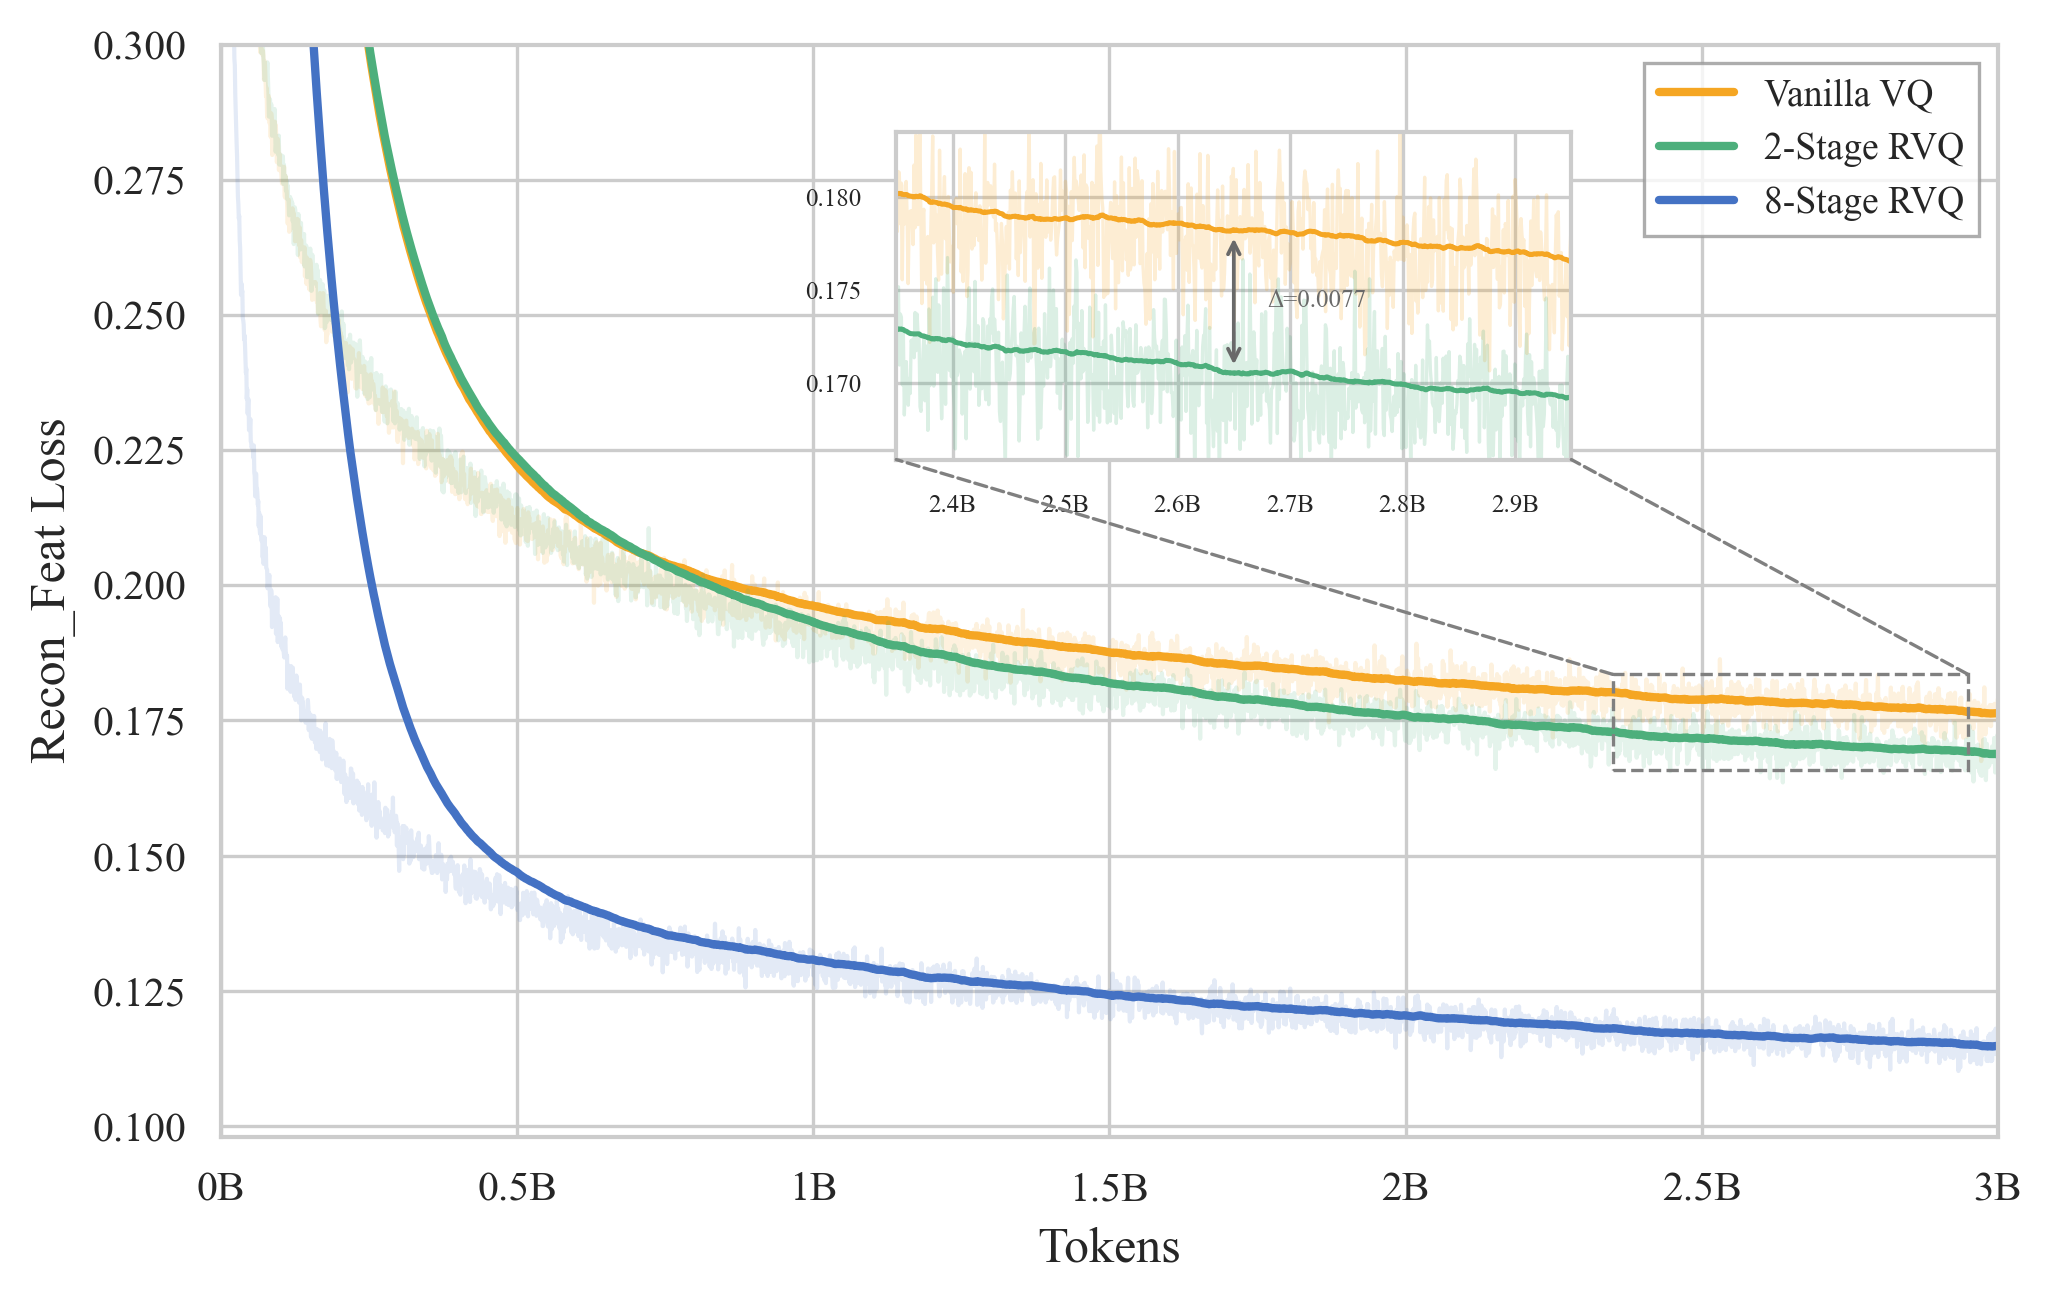
\includegraphics[width=0.8\linewidth]{figs/rvq_loss.png}
%     \caption{Comparison of feature reconstruction loss across different discrete quantization strategies.}
%     \label{fig:rvq_loss}
% \end{figure}

